
% ME3050 -  Dynamics Modeling and Controls - Tennessee Technological University
% Tristan Hill - Spring 2020 - Summer 2020 - Spring 2022
% Dynamics Modeling and Controls
% Lecture Module - Laplace Transforms - Topic 1  - Definition of the Laplace Transform 

% Document settings

%\documentclass{beamer}                  % for presentation ?
\documentclass[handout]{beamer}  % for handout ?

\usepackage{/home/thill/Documents/lectures/dmc_lectures/dmc_lectures}

%\newcommand{\MNUM}{10\hspace{2mm}} % Module number
\newcommand{\TNUM}{1\hspace{2mm}} % Topic number 
\newcommand{\moduletitle}{The Laplace Transform} % Titles and Stuff
\newcommand{\topictitle}{Definition of the Laplace Transform} 

\newcommand{\sectiontitleI}{An Integral Transform} % More Titles and Stuff
\newcommand{\sectiontitleII}{Laplace Transform of A Derivative}
\newcommand{\sectiontitleIII}{Properties of an Integral}
\newcommand{\sectiontitleIV}{Table of Transform Pairs}

\author{ME3050 - Dynamic Modeling and Controls}
\title{Lecture Module - \moduletitle}
\date{Mechanical Engineering\vspc Tennessee Technological University}

\begin{document}
	
	\lstset{language=MATLAB,basicstyle=\ttfamily\small,showstringspaces=false}
	
	\frame{\titlepage \center\begin{framed}\Large \textbf{Topic \TNUM - \topictitle}\end{framed} \vspace{5mm}}
	
	% Section 0 - Outline
	\frame{
		
		\large \textbf{Topic \TNUM - \topictitle} \vspace{3mm}\\
		
		\begin{itemize}
			
			\item \sectiontitleI    \vspc % Section I
			\item \sectiontitleII 	\vspc % Section II
			\item \sectiontitleIII 	\vspc %Section III
			\item \sectiontitleIV 	\vspc %Section IV
			%\item \sectiontitleV 	\vspc %Section V
			
		\end{itemize}
		
	}


\section{\sectiontitleI}

\frame{ 
\frametitle{\sectiontitleI}

The Laplace Transform is an Integral Transform

Given a function $x(t)$ in the time domain where $t\geq0$, \\ the Laplace Transform is defined as follows: \\

\[ X(s)=\Lagr{\{x(t)\}}=\displaystyle\int_0^{\infty} x(t)e^{-st}dt \]

And its inverse is similarly defined as: \\

\[ \Lagr^{-1}{\{X(s)\}}=x(t) \]

The Laplace Domain variable $s$ is a complex number: \[ s=\sigma+j\omega \] 

}




\section{\sectiontitleII}
\frame{
\frametitle{\sectiontitleII}



It is useful to find the laplace transform of the derivative of a function: 
\[ \Lagr{\{\frac{d}{dt}(x(t))\} }=\Lagr{\{\dot{x}(t)\}} =s\Lagr{\{x(t)\} }-x(t=0) \]
\[ \hspace{52mm} =sX(s)-x(t=0) \]
\[ \hspace{52mm}\Lagr{\{ \dot{x} \left(t\right) \}} =sX(s)-x_0 \]

\[ \Lagr{\{\frac{d^2}{dt^2}(x(t))\} }=\Lagr{\{\ddot{x}(t)\}} = s^2\Lagr{\{x(t)\} }-sx(t=0)-\dot{x}(t=0) \]
\[ \hspace{52mm} = s^2X(s)-sx(t=0)-\dot{x}(t=0) \]
\[ \hspace{52mm} \Lagr{\{ \ddot{x} \left(t\right) \}}= s^2X(s)-sx_0-\dot{x}_0  \]


}

\section{\sectiontitleIII}
\frame{
\frametitle{\sectiontitleIII}

Also, remember that the transform inherits the properties of an integral.

\[ \int\left[ x(t)+y(t) \right]dt =\int x(t)dt + \int y(t)dt \]
\[ \int Kx(t)dt = K\int x(t)dt \hspcc (K \hspc is \hspc constant)\]

Therefore these properties can be used with the Laplace transform.
}

\section{\sectiontitleIV}
\frame{
\frametitle{\sectiontitleIV}

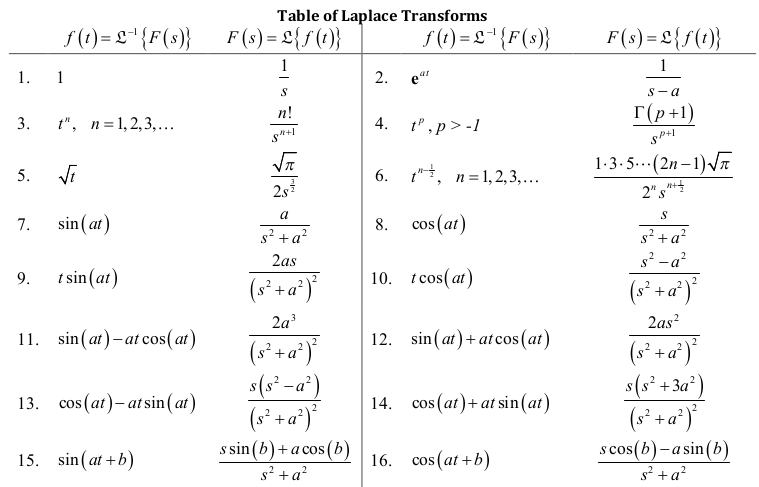
\includegraphics[scale=.35]{laplace_table_part1.png}


}

\frame{
\frametitle{\sectiontitleIV}

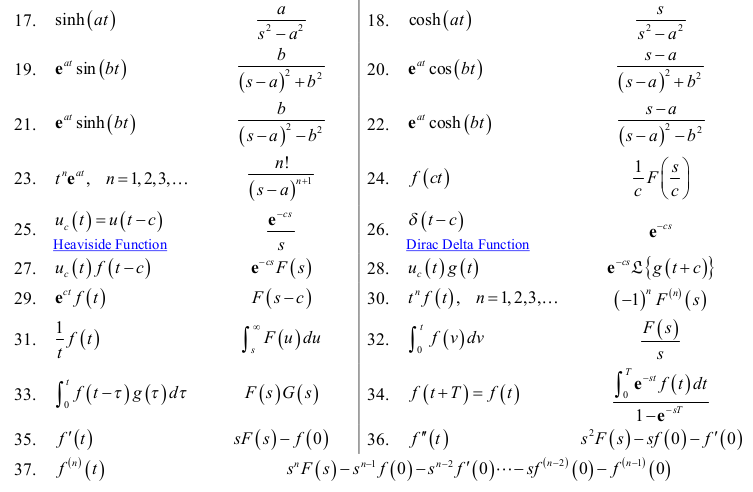
\includegraphics[scale=.35]{laplace_table_part2.png}


}

\section{---}
\frame{
\frametitle{---}

Why use or learn this method? \vspc


}

\end{document}

